\appendix
\chapter{Physics analysis}
\section{Quark-gluon discriminator study}

The $p_{t}D$ in terms of jet $\eta$ in different jet flavors is showed in Fig~\ref{fig:c4ttqgptdjeteta}.
\begin{figure}[htbp]
 \begin{center}
  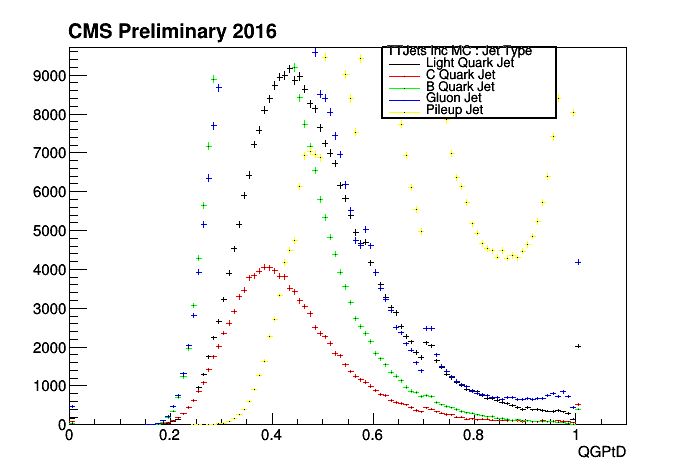
\includegraphics[width=0.45\textwidth]{sections/mc4/TopTagger/figures/_b_qgptdjetetabin0_.png}
  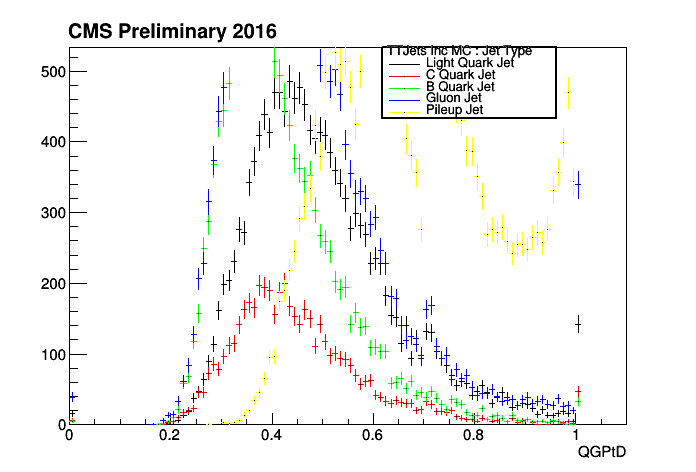
\includegraphics[width=0.45\textwidth]{sections/mc4/TopTagger/figures/_b_qgptdjetetabin1_.png} \\
  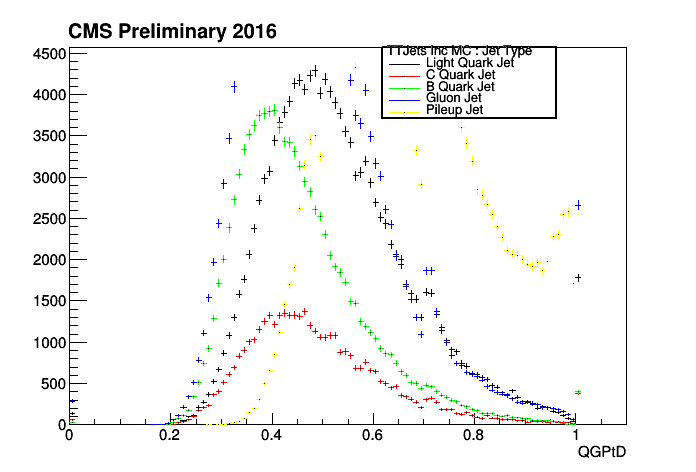
\includegraphics[width=0.45\textwidth]{sections/mc4/TopTagger/figures/_b_qgptdjetetabin2_.png}
  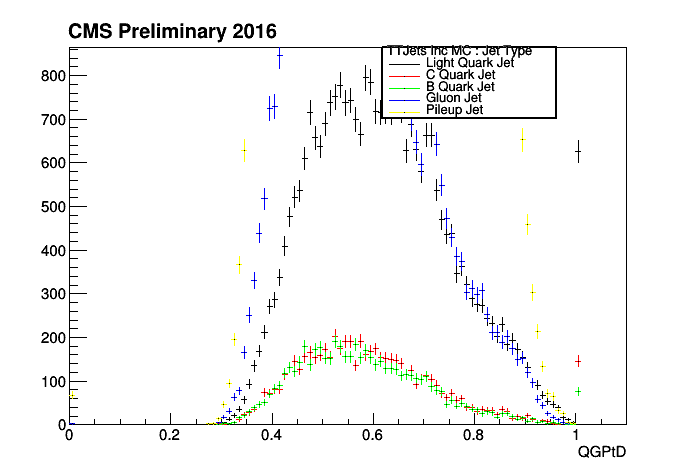
\includegraphics[width=0.45\textwidth]{sections/mc4/TopTagger/figures/_b_qgptdjetetabin3_.png} \\
  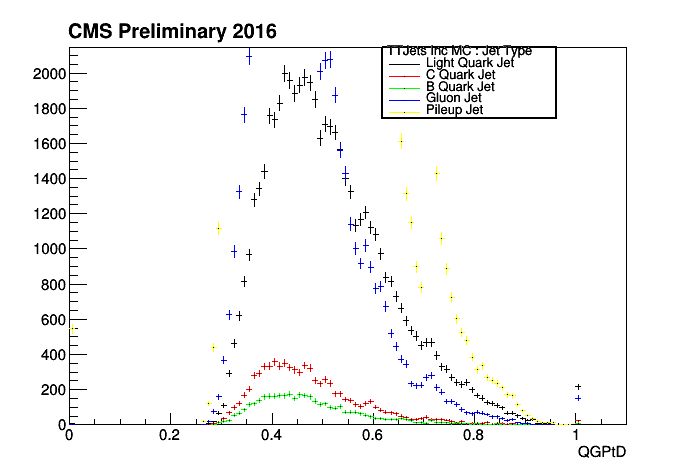
\includegraphics[width=0.45\textwidth]{sections/mc4/TopTagger/figures/_b_qgptdjetetabin4_.png}
  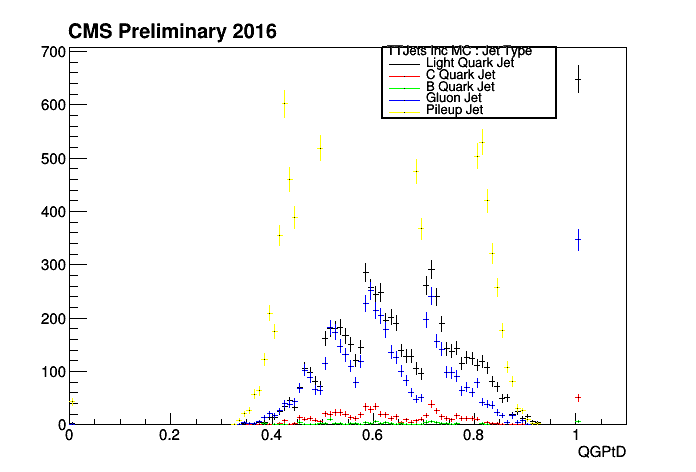
\includegraphics[width=0.45\textwidth]{sections/mc4/TopTagger/figures/_b_qgptdjetetabin5_.png}
 \end{center}
 \caption{Top left: Quark Gluon $p_{t}D$ for jet $\eta$ bin 1; Top right: jet $\eta$ bin 2; Middle left: jet $\eta$ bin 3; Middle right: jet $\eta$ bin 4; Middle left: jet $\eta$ bin 5; Middle right: jet $\eta$ bin 6}
 \label{fig:c4ttqgptdjeteta}
\end{figure}

The $p_{t}D$ in terms of jet $p_{T}$ in different jet flavors is showed in Fig~\ref{fig:c4ttqgptdjetpt}.
\begin{figure}[htbp]
 \begin{center}
  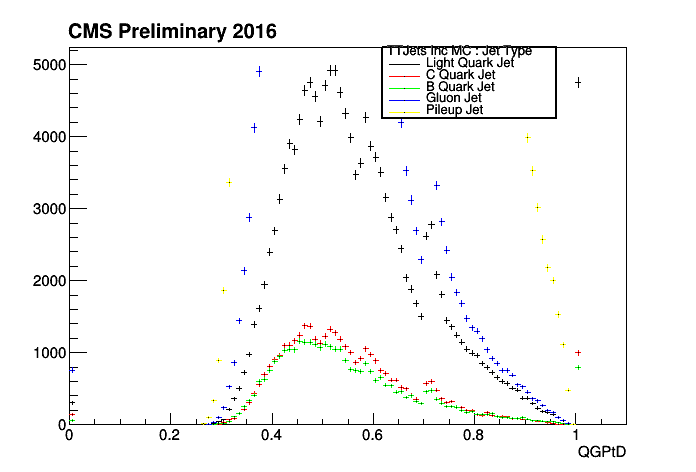
\includegraphics[width=0.45\textwidth]{sections/mc4/TopTagger/figures/_b_qgptdjetptbin0_.png}
  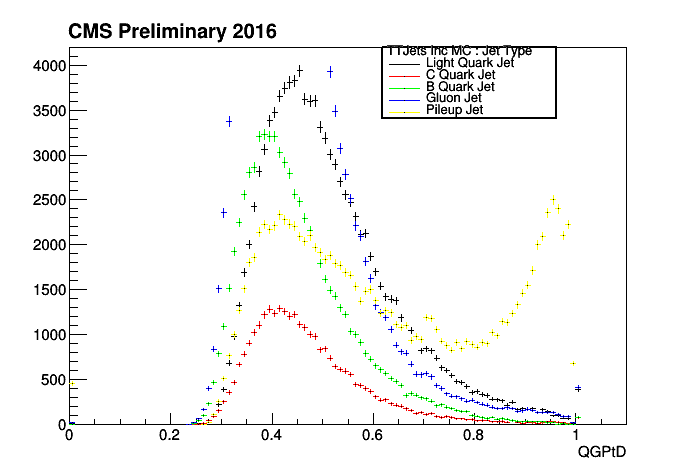
\includegraphics[width=0.45\textwidth]{sections/mc4/TopTagger/figures/_b_qgptdjetptbin1_.png} \\
  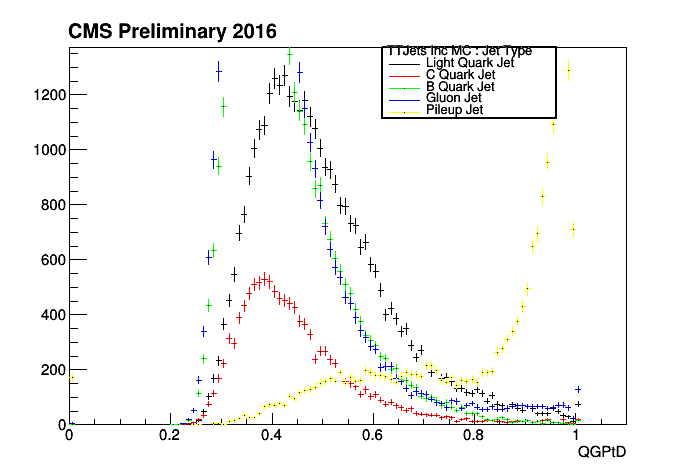
\includegraphics[width=0.45\textwidth]{sections/mc4/TopTagger/figures/_b_qgptdjetptbin2_.png}
  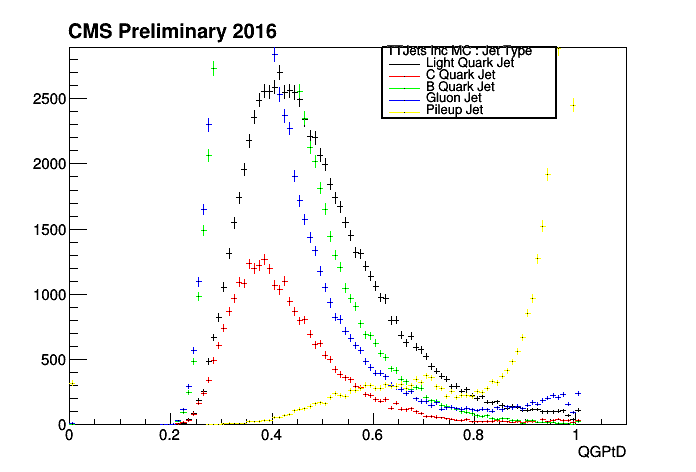
\includegraphics[width=0.45\textwidth]{sections/mc4/TopTagger/figures/_b_qgptdjetptbin3_.png} \\
  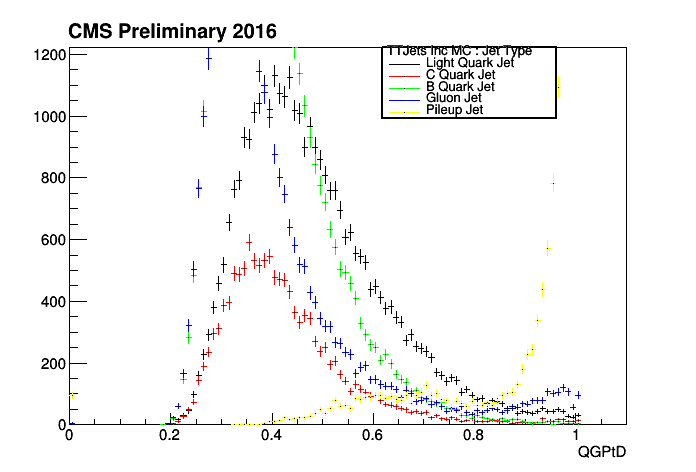
\includegraphics[width=0.45\textwidth]{sections/mc4/TopTagger/figures/_b_qgptdjetptbin4_.png}
  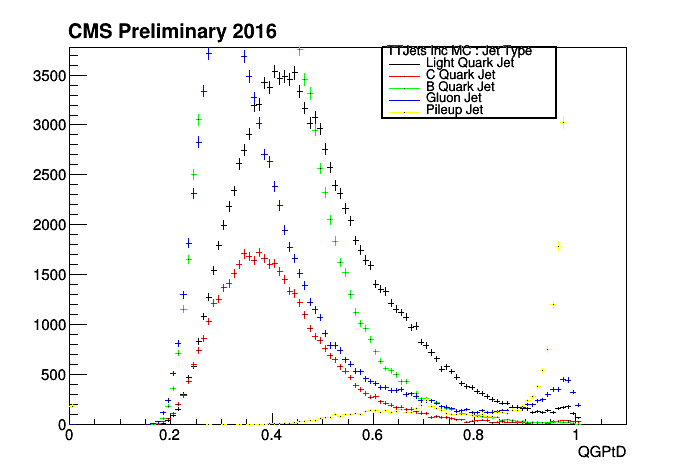
\includegraphics[width=0.45\textwidth]{sections/mc4/TopTagger/figures/_b_qgptdjetptbin5_.png}
 \end{center}
 \caption{Top left: Quark Gluon $p_{t}D$ for jet $p_{T}$ bin 1; Top right: jet $p_{T}$ bin 2; Middle left: jet $p_{T}$ bin 3; Middle right: jet $p_{T}$ bin 4; Middle left: jet $p_{T}$ bin 5; Middle right: jet $p_{T}$ bin 6}
 \label{fig:c4ttqgptdjetpt}
\end{figure}

The multiplicity in terms of jet $\eta$ in different jet flavors is showed in Fig~\ref{fig:c4ttqgmultjeteta}.
\begin{figure}[htbp]
 \begin{center}
  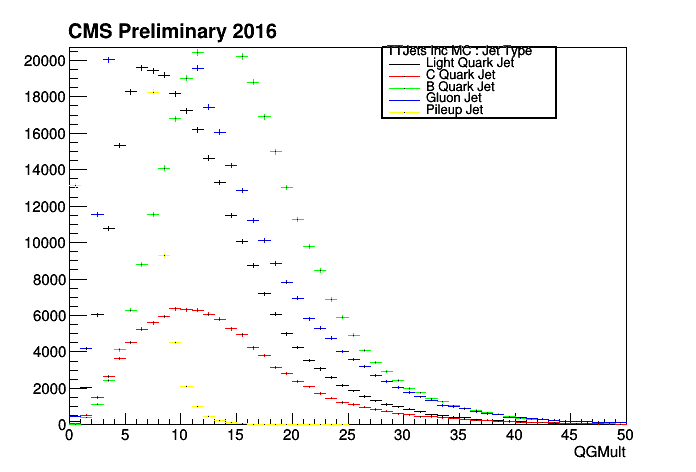
\includegraphics[width=0.45\textwidth]{sections/mc4/TopTagger/figures/_b_qgmultjetetabin0_.png}
  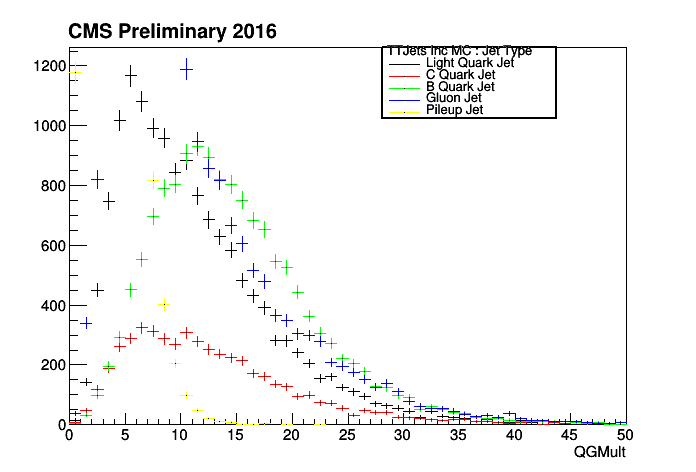
\includegraphics[width=0.45\textwidth]{sections/mc4/TopTagger/figures/_b_qgmultjetetabin1_.png} \\
  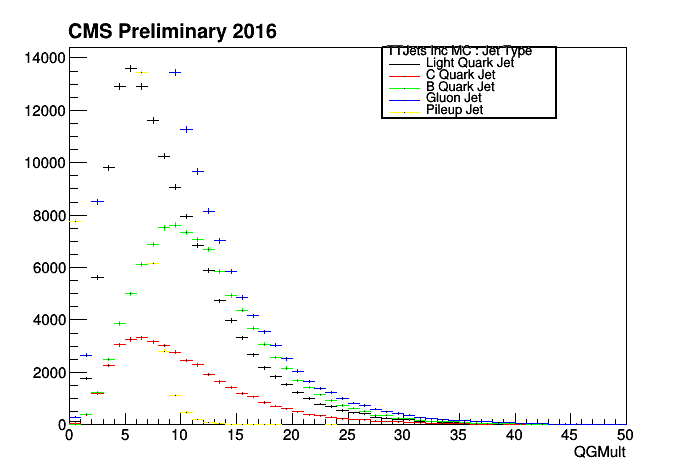
\includegraphics[width=0.45\textwidth]{sections/mc4/TopTagger/figures/_b_qgmultjetetabin2_.png}
  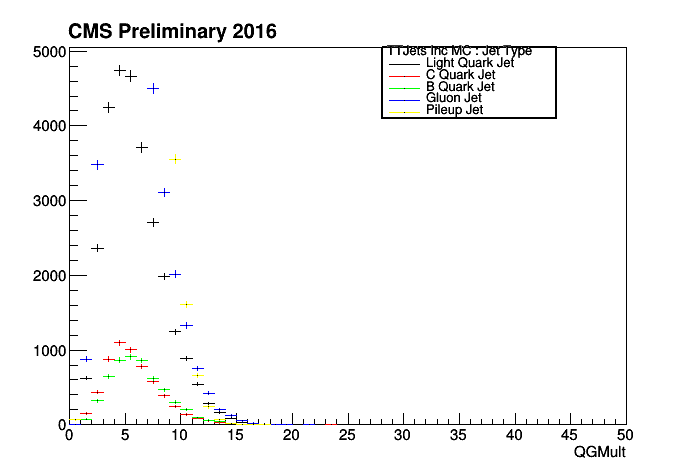
\includegraphics[width=0.45\textwidth]{sections/mc4/TopTagger/figures/_b_qgmultjetetabin3_.png} \\
  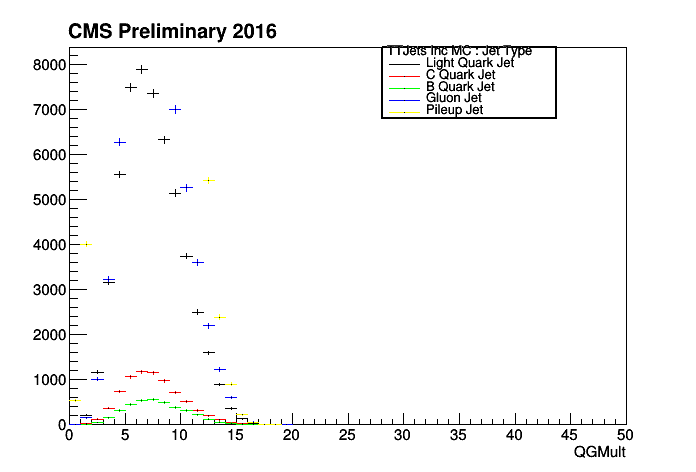
\includegraphics[width=0.45\textwidth]{sections/mc4/TopTagger/figures/_b_qgmultjetetabin4_.png}
  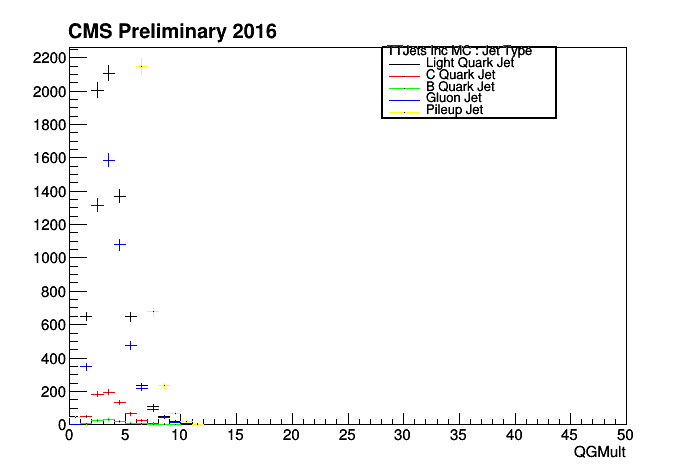
\includegraphics[width=0.45\textwidth]{sections/mc4/TopTagger/figures/_b_qgmultjetetabin5_.png}
 \end{center}
 \caption{Top left: Quark Gluon multiplicity for jet $\eta$ bin 1; Top right: jet $\eta$ bin 2; Middle left: jet $\eta$ bin 3; Middle right: jet $\eta$ bin 4; Middle left: jet $\eta$ bin 5; Middle right: jet $\eta$ bin 6}
 \label{fig:c4ttqgmultjeteta}
\end{figure}

The multiplicity in terms of jet $p_{T}$ in different jet flavors is showed in Fig~\ref{fig:c4ttqgmultjetpt}.
\begin{figure}[htbp]
 \begin{center}
  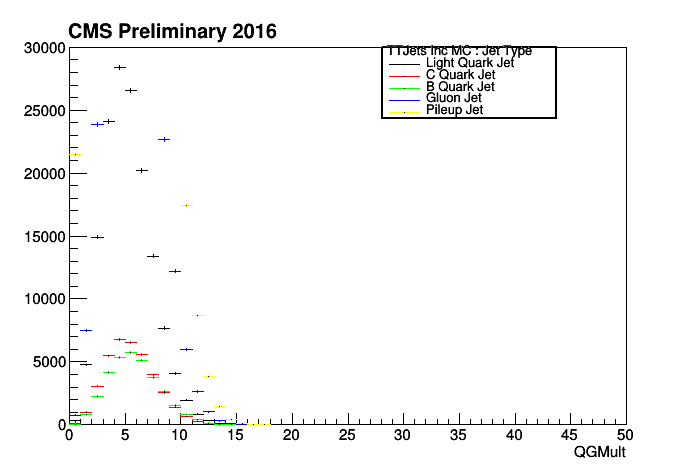
\includegraphics[width=0.45\textwidth]{sections/mc4/TopTagger/figures/_b_qgmultjetptbin0_.png}
  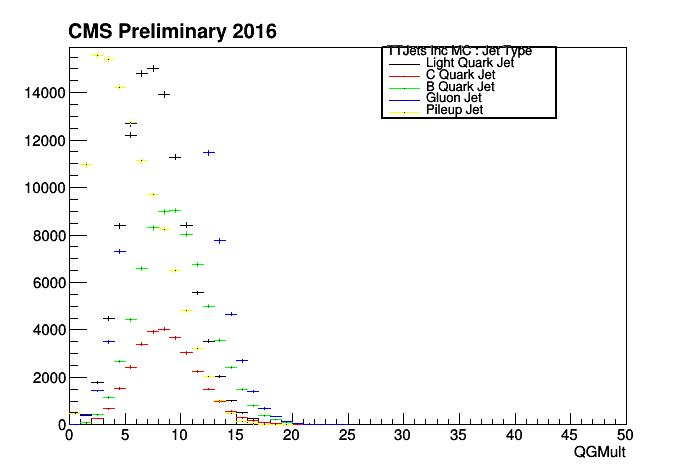
\includegraphics[width=0.45\textwidth]{sections/mc4/TopTagger/figures/_b_qgmultjetptbin1_.png} \\
  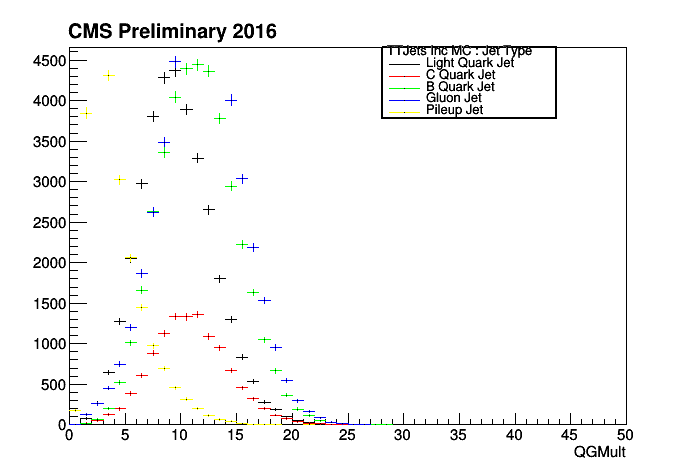
\includegraphics[width=0.45\textwidth]{sections/mc4/TopTagger/figures/_b_qgmultjetptbin2_.png}
  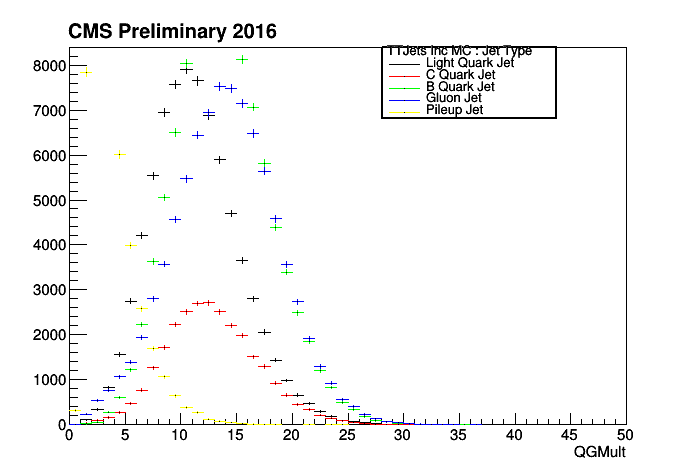
\includegraphics[width=0.45\textwidth]{sections/mc4/TopTagger/figures/_b_qgmultjetptbin3_.png} \\
  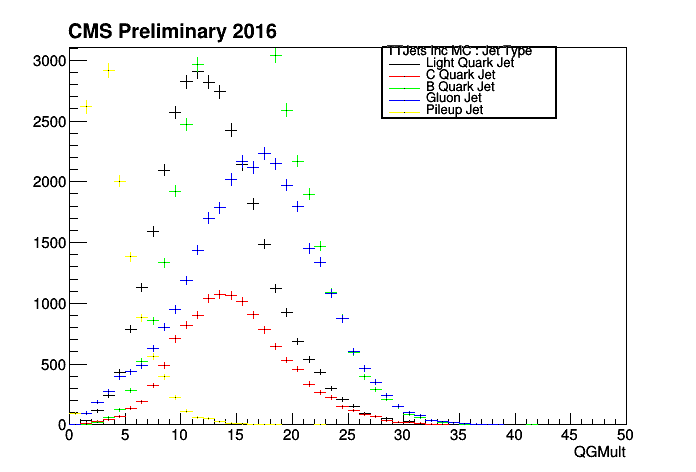
\includegraphics[width=0.45\textwidth]{sections/mc4/TopTagger/figures/_b_qgmultjetptbin4_.png}
  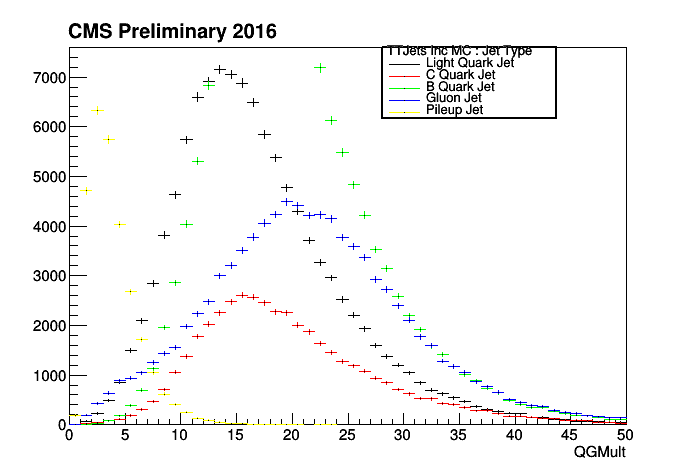
\includegraphics[width=0.45\textwidth]{sections/mc4/TopTagger/figures/_b_qgmultjetptbin5_.png}
 \end{center}
 \caption{Top left: Quark Gluon multiplicity for jet $p_{T}$ bin 1; Top right: jet $p_{T}$ bin 2; Middle left: jet $p_{T}$ bin 3; Middle right: jet $p_{T}$ bin 4; Middle left: jet $p_{T}$ bin 5; Middle right: jet $p_{T}$ bin 6}
 \label{fig:c4ttqgmultjetpt}
\end{figure}

The Axis2 in terms of jet $\eta$ in different jet flavors is showed in Fig~\ref{fig:c4ttqgaxis2jeteta}.
\begin{figure}[htbp]
 \begin{center}
  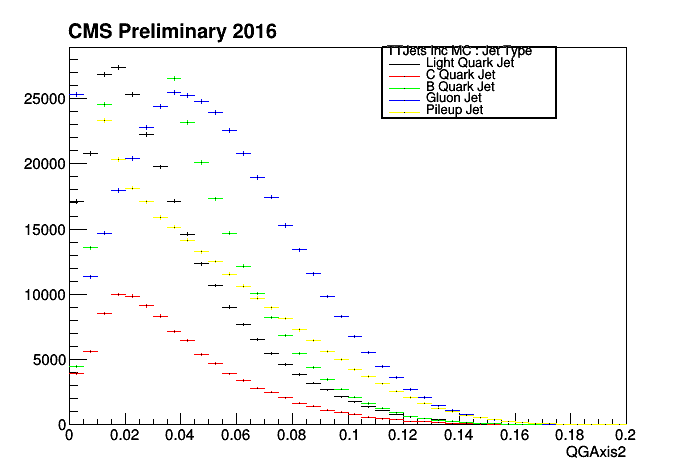
\includegraphics[width=0.45\textwidth]{sections/mc4/TopTagger/figures/_b_qgaxis2jetetabin0_.png}
  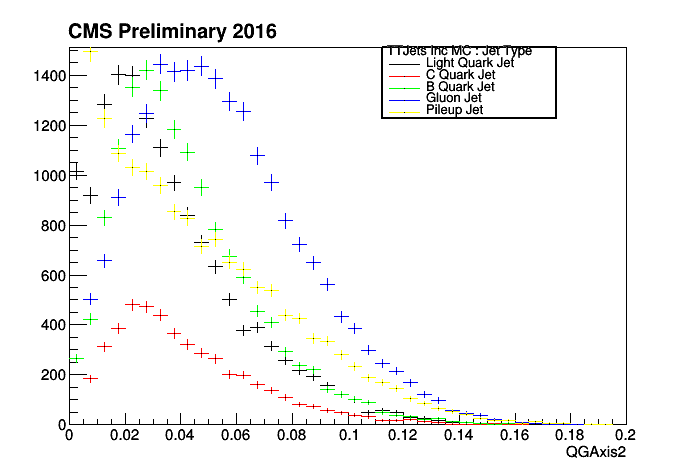
\includegraphics[width=0.45\textwidth]{sections/mc4/TopTagger/figures/_b_qgaxis2jetetabin1_.png} \\
  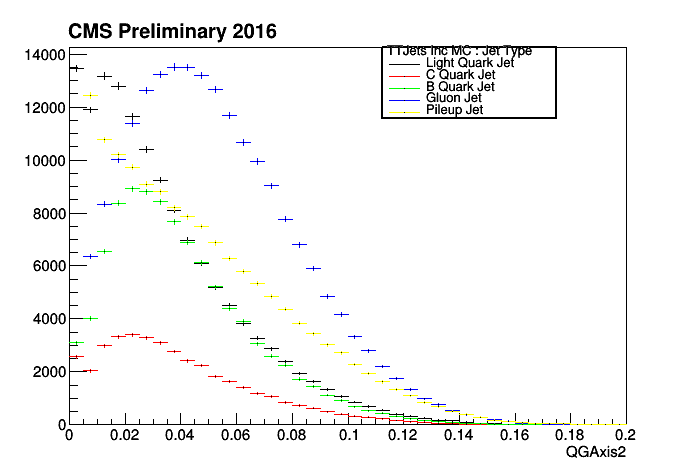
\includegraphics[width=0.45\textwidth]{sections/mc4/TopTagger/figures/_b_qgaxis2jetetabin2_.png}
  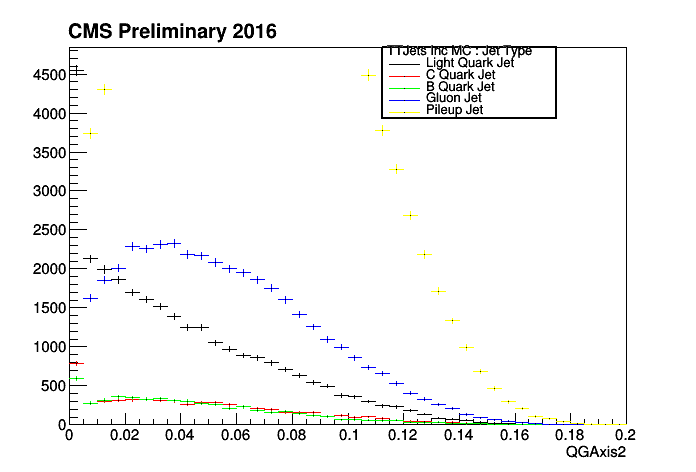
\includegraphics[width=0.45\textwidth]{sections/mc4/TopTagger/figures/_b_qgaxis2jetetabin3_.png} \\
  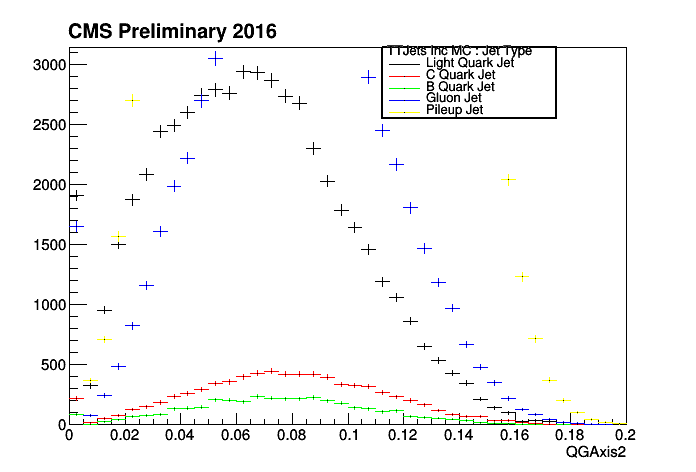
\includegraphics[width=0.45\textwidth]{sections/mc4/TopTagger/figures/_b_qgaxis2jetetabin4_.png}
  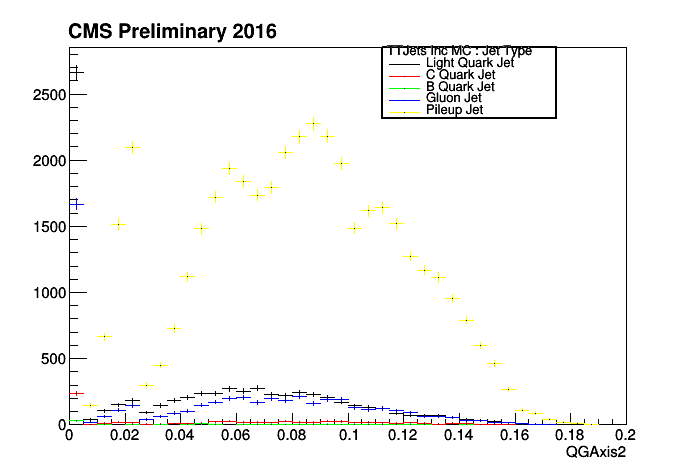
\includegraphics[width=0.45\textwidth]{sections/mc4/TopTagger/figures/_b_qgaxis2jetetabin5_.png}
 \end{center}
 \caption{Top left: Quark Gluon Axis2 for jet $\eta$ bin 1; Top right: jet $\eta$ bin 2; Middle left: jet $\eta$ bin 3; Middle right: jet $\eta$ bin 4; Middle left: jet $\eta$ bin 5; Middle right: jet $\eta$ bin 6}
 \label{fig:c4ttqgaxis2jeteta}
\end{figure}

The Axis2 in terms of jet $p_{T}$ in different jet flavors is showed in Fig~\ref{fig:c4ttqgaxis2jetpt}.
\begin{figure}[htbp]
 \begin{center}
  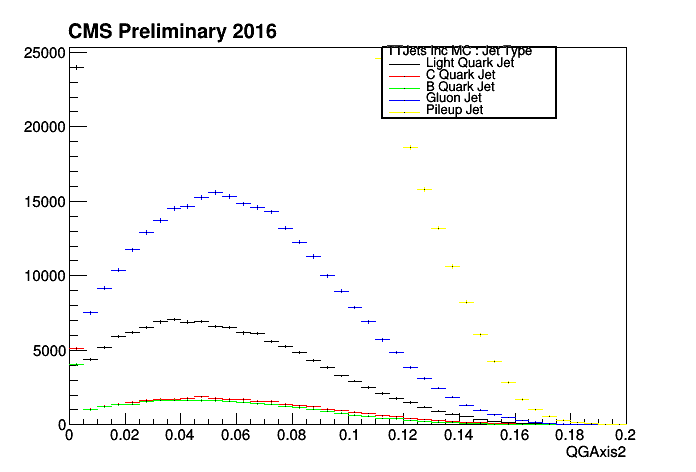
\includegraphics[width=0.45\textwidth]{sections/mc4/TopTagger/figures/_b_qgaxis2jetptbin0_.png}
  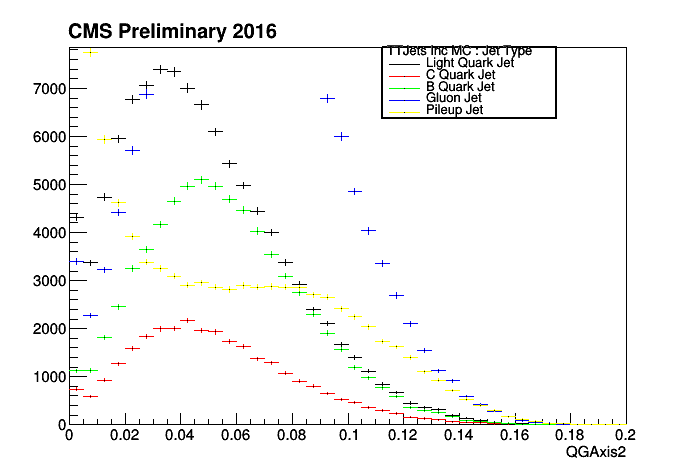
\includegraphics[width=0.45\textwidth]{sections/mc4/TopTagger/figures/_b_qgaxis2jetptbin1_.png} \\
  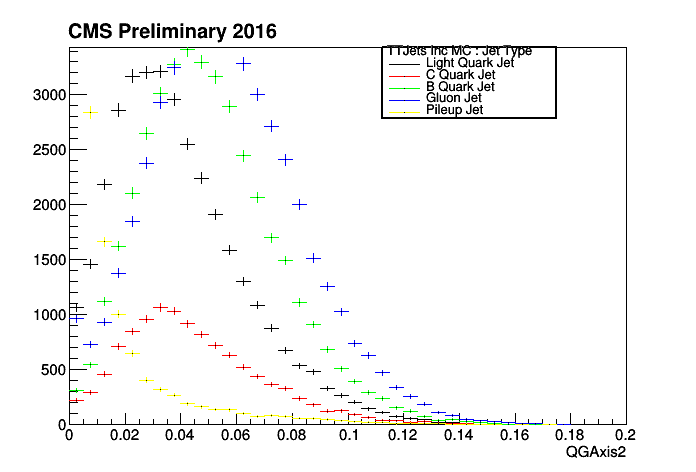
\includegraphics[width=0.45\textwidth]{sections/mc4/TopTagger/figures/_b_qgaxis2jetptbin2_.png}
  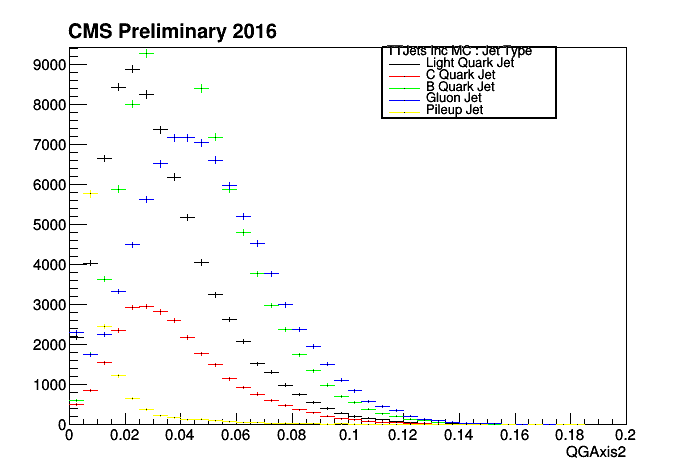
\includegraphics[width=0.45\textwidth]{sections/mc4/TopTagger/figures/_b_qgaxis2jetptbin3_.png} \\
  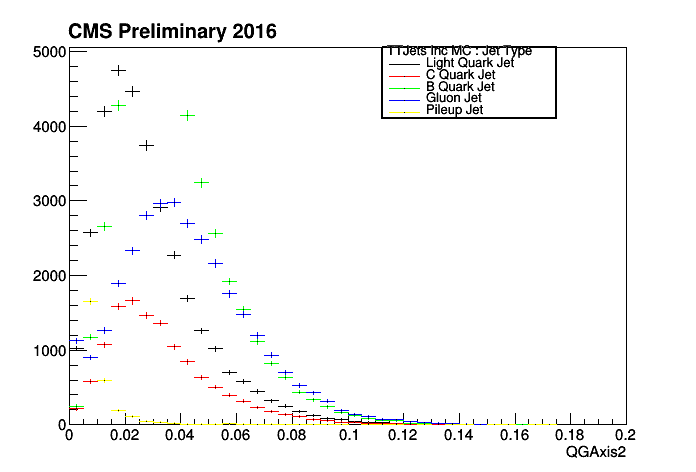
\includegraphics[width=0.45\textwidth]{sections/mc4/TopTagger/figures/_b_qgaxis2jetptbin4_.png}
  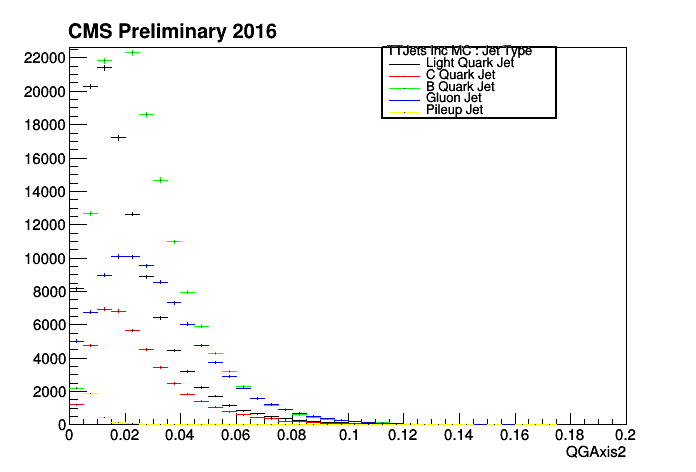
\includegraphics[width=0.45\textwidth]{sections/mc4/TopTagger/figures/_b_qgaxis2jetptbin5_.png}
 \end{center}
 \caption{Top left: Quark Gluon Axis2 for jet $p_{T}$ bin 1; Top right: jet $p_{T}$ bin 2; Middle left: jet $p_{T}$ bin 3; Middle right: jet $p_{T}$ bin 4; Middle left: jet $p_{T}$ bin 5; Middle right: jet $p_{T}$ bin 6}
 \label{fig:c4ttqgaxis2jetpt}
\end{figure}

\section{Di-Top jets event display}
The Event with two reconstructed top jets are demonstrated in Fig~\ref{fig:appttevtdisplay}. The jet energies and \MET shown are without energy correction.
\begin{figure}[htbp]
 \begin{center}
  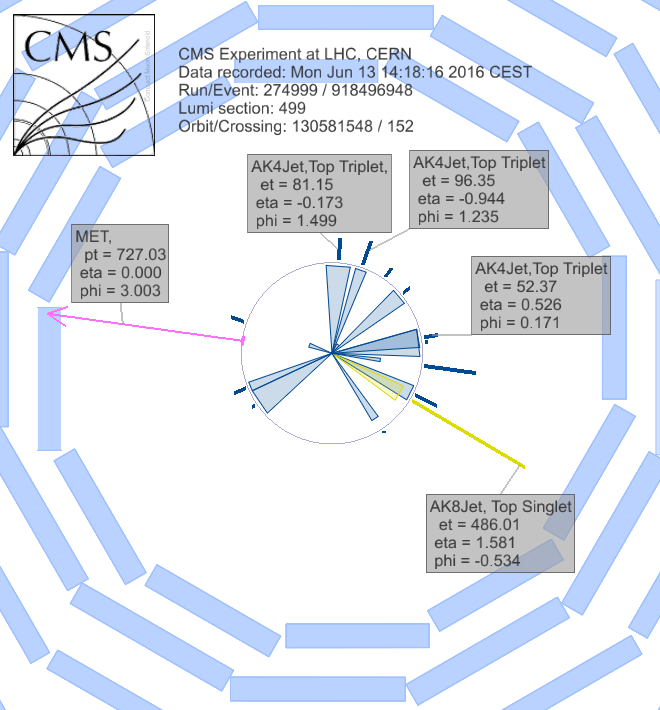
\includegraphics[width=0.45\textwidth]{figures/appendix/appendix_tagger_Run2016B_2t_1j3j-274999_918496948_499_RhoPhi.png}
  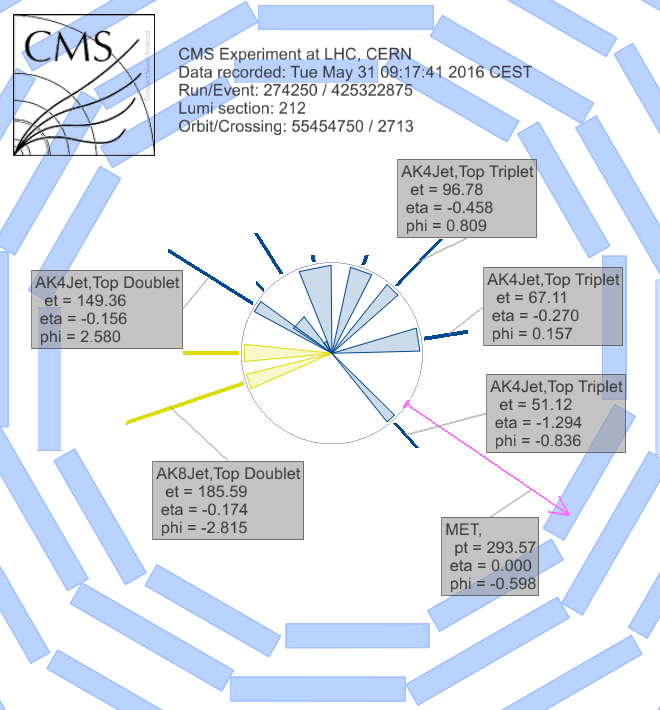
\includegraphics[width=0.45\textwidth]{figures/appendix/appendix_tagger_Run2016B_2t_2j3j-274250_425322875_212_RhoPhi.png}
\end{center} \caption{Event display for di-topjets event in data. Left plot is one mono-jet top and one triple-jet top, Right plot is one di-jet top and one triple-jet top. Yellow line is fat jet (anti-$k_{T}$ R=0.8), blue line is normal jet (anti-$k_{T}$ R=0.4), the purple line is \MET.}
 \label{fig:appttevtdisplay}
\end{figure}

\section{Aggregate search bin, simplified top tagger and results}

